\section{The Transformer Architecture}

\subsection{Standard Transformers}

We consider transformer networks~\citep{Vaswani_A_2017_p-nips-OG} composed of repeated self-attention and MLP layers, together with an embedding layer and a final linear projection.

\begin{definition}[One-Hot Representation]
Let $\mathcal V=\{t_1,\ldots,t_{|\mathcal V|}\}$ denote the vocabulary.  
For a token $t_i\in\mathcal V$, the \emph{one-hot representation} of $t_i$ is the canonical vector 
\[
\mathbf c_i=(\mathbf1_{i=j})_{j\in[|\mathcal V|]}\in\mathbb R^{|\mathcal V|}.
\]
\end{definition}


\begin{definition}[Embedding Layer]
Let $\mathbf{E}\in\mathbb R^{d\times |\mathcal{V}|}$ be the embedding matrix.  
For a sequence of $m$ tokens $\mathbf{t}=(t_{i_1},\ldots,t_{i_m})\in\mathcal{V}^m$, the embedding layer maps the one-hot representation $[\mathbf c_{i_1},\ldots,\mathbf c_{i_m}]\in\mathbb R^{|\mathcal V|\times m}$ to
\[
\mathbf{X}_{\mathbf t} = \mathbf{E}[\mathbf c_{i_1},\ldots,\mathbf c_{i_m}]\in\mathbb R^{d\times m}.
\]
\end{definition}

\begin{definition}[Transformer with Hard Prompt Inputs]\label{def:hard_prompt}
    An $l$-layer transformer with vocabulary $\mathcal V$ and unembedding matrix $\mathbf F\in\mathbb R^{|\mathcal{V}|\times d}$ is the mapping
    \[
    \tau:\bigcup_{m=1}^{+\infty}\mathcal{V}^m \longrightarrow \Delta^{\mathcal{V}},
    \]
    defined as
    \begin{align*}
        &\tau(\mathbf{t}) = \sigma\big( \mathbf F (\mathbf{X}_l)_{:,-1} \big),\quad\mbox{where}\\
    &\mathbf{X}_l = \mathrm L(\mathbf{X}_{\mathbf t})\quad\mbox{is the output of the final transformer layer,}\\
    &\mathbf{X}_{\mathbf t}\quad\mbox{is the embedded input with positional encodings.}
    \end{align*}

    The only characteristic of the transformer layers $\mathrm L$ required in this paper is that they keep the embedding space bounded. The formal proof and empirical validation, together with the formal definition of $\mathrm L$ are deferred to Appendix~\ref{app:transformer_layer}.
\end{definition}

A transformer can also be seen as mapping soft prompt inputs from $\bigcup_{m=1}^{+\infty}\mathbb{R}^{d\times m}$ (which may or may not correspond to sequences of tokens).

\begin{definition}[Transformer with Soft Prompt Inputs]\label{def:soft_prompt}
     An $l$-layer transformer with embedding dimension $d$ is the mapping
    \[
    \tau:\bigcup_{m=1}^{+\infty}\mathbb R^{d\times m} \longrightarrow \Delta^{\mathcal{V}},
    \]
    defined as
    \begin{align*}
        &\tau(\mathbf{X}) = \sigma\Big( \mathbf F\big( \mathrm L(\mathbf{X})\big)_{:,-1} \Big).
    \end{align*}
\end{definition}

We consider Definition~\ref{def:soft_prompt} in our analysis. However, since a transformer with soft prompt inputs is more expressive than its hard prompt counterpart, all of our results directly extend to Definition~\ref{def:hard_prompt}.

\subsection{Mean-Field Transformers}\label{sec:mean-field}

To handle arbitrary prompt lengths, we can interpret transformers as maps over probability measures~\citep{pmlr-v151-sander22a,NEURIPS2023_b2b3e1d9}. This is possible because of two key properties of attention (and hence of a transformer as defined in Definition~\ref{def:soft_prompt}):
\begin{itemize}
    \item Attention layers are permutation equivariant.
    \item For any attention block $\mathrm L$ and input $\mathbf X$, $\mathrm L(\mathbf X)_{:,i}=\mathrm L([\mathbf X,\mathbf X])_{:,i}$.
\end{itemize}

We can thus replace every sequence \( \mathbf X \) of length $m$ with its associated empirical measure
\[
\mathrm{M}(\mathbf X) := \frac{1}{m} \sum_{i=1}^m \delta_{\mathbf X_{:,i}},
\]

\begin{figure*}[!ht]
    \centering
    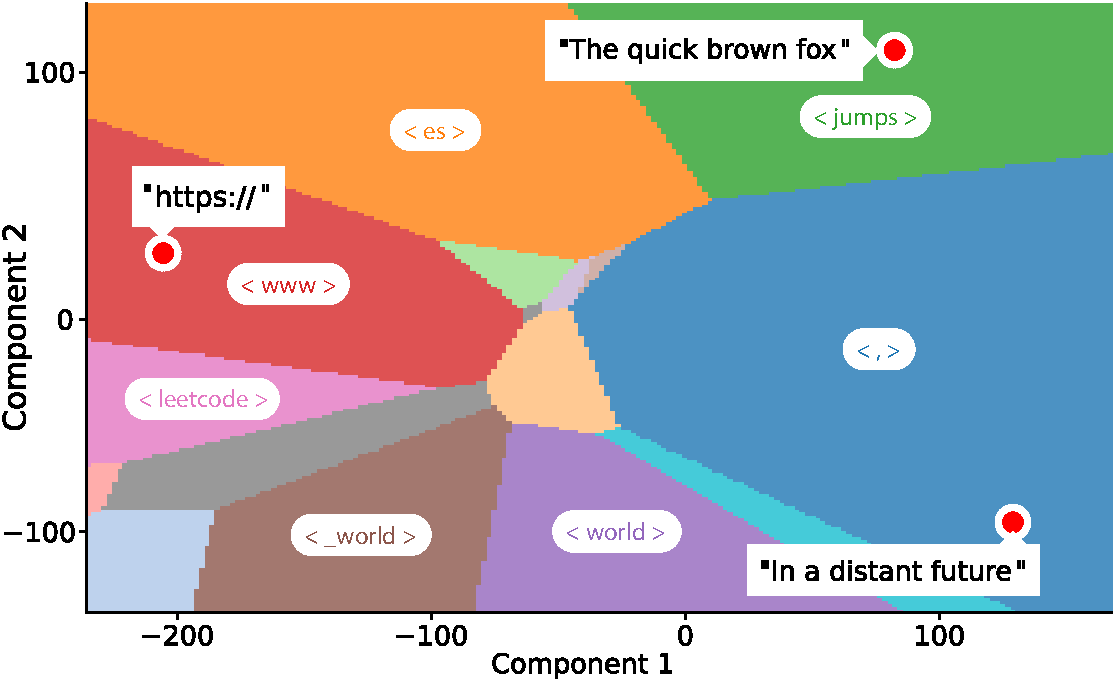
\includegraphics[width=0.6\textwidth]{Images/qwen_token_plane_visualization2.pdf}
    \caption{Plane cut of the embedding space $\mathcal{E}$ of Qwen-2~(0.5B)~\citep{yang2024qwen2}, passing through the final token embeddings of “The quick brown fox”, “https://”, and “In a distant future” (red markers).
    Colors encode, for each pixel, the most probable next token via the model’s output projection (decoder readout). This induces regions $\mathcal{E}_{\mathrm t}$ annotated by $<\mathrm t>$. Only tokens whose regions have the largest areas are annotated for readability. The three embeddings fall respectively in $\mathcal{E}_{\text{jumps}}$, $\mathcal{E}_{\text{www}}$, and $\mathcal{E}_{,}$, {\it i.e.} the predicted next tokens are $<$jumps$>$, $<$www$>$, and $<$,$>$.}
    \label{fig:next_token}
\vspace{-0.5em}
\end{figure*}


so that a transformer can be viewed as a transformation of probability measures supported on \( \mathbb{R}^d \), independent of the ordering of tokens. This is called the mean-field extension of transformers, and we describe it further in Appendix~\ref{app:mean_field}.

\begin{remark}[Positional Encodings and Masked Attention]
    The mean-field framework can also be extended to most types of positional encodings and to masked attention, as discussed in Appendix~\ref{app:mean_field}.
\end{remark}
